% $Id: conclusion.tex 
% !TEX root = main.tex

%%
\section{Background}
\label{sec:background}

%%%%
\subsection{\acl{RL}}

In \ac{RL}, agents learn to map environmental situations (environment states) to actions that maximize a numerical reward signal received from the environment in the long term~\cite{sutton18}. \ac{RL} problems are formulated as Markov Decision Processes (MDPs), defined by the tuple $\mathcal{M} = \langle \mathcal{S}, \mathcal{A}, P, R, \gamma \rangle$, where:
$\mathcal{S}$ is the state space, comprising all relevant states of the environment;
$\mathcal{A}$ is the action space, i.e., the set of all actions the agent can perform to affect the environment;
$P(s_{t+1} \mid s_t, a_t)$ is the transition probability from state {\color{purple}$s_t$} to {\color{purple}$s_{t+1}$} under action {\color{purple}$a_t$};
$R(s_t, a_t)$ is the reward function, providing the numerical signal ($r$) that encodes the positive or negative impact of taking action {\color{purple}$a_t$} in state {\color{purple}$s_t$} at each execution step $t$; and $\gamma \in [0, 1]$ is the discount factor, which determines the importance of future rewards.

In stationary settings, $P$ and $R$ remain fixed over time, and the agent’s objective is to learn a policy $\pi: \mathcal{S} \to \mathcal{A}$ that maximizes the expected discounted return. However, real-world environments often violate this stationarity assumption: transition dynamics and/or reward functions may shift due to evolving conditions. We model such scenarios as \emph{non-stationary} MDPs, represented by a sequence
\[
\{\mathcal{M}_t\}_{t=1}^\infty
\quad\text{with}\quad
\mathcal{M}_t = \bigl\langle \mathcal{S}, \mathcal{A}_t, P_t, R_t, \gamma \bigr\rangle,
\]
where $P_t$ and/or $R_t$ change at unknown time steps $t$ (``concept drifts''). In this work, we further consider the novel scenario where the agent's action space $\mathcal{A}$ may also change over time. Detecting and adapting to these drifts is central to \ac{CRL}~\cite{khetarpal2022continualreinforcementlearningreview,abel2023definitioncontinualreinforcementlearning}, which treats learning as an ongoing process across a continually changing sequence of tasks.

Q-learning~\cite{watkins92} is a widely used model-free approach in \ac{RL}. The long-term quality of an action performed at a given state is computed iteratively in a series of steps and is represented by a Q value,
$\mathit{Q(s,a)}$.
Formally, each execution step $t$ captures information from the environment and maps it to a state
{\color{purple}$s_t$} $\in \mathcal{S}$ in its state space. It then selects an
action {\color{purple}$a_t$} $\in \mathcal{A}$ from its action space and executes it. The agent
receives a reward {\color{Bittersweet}$r_t$} from the environment when it moves to the next state
$s_{t+1} \in \mathcal{S}$. The reward is used to update the optimality of performing the
action {\color{Mulberry}$a_t$} at state {\color{purple}$s_t$}. The agent's goal is to learn
a policy (\i.e. the best-fit action for each state) that maximizes the reward of the
long-run behavior. The learning rate \lrate{\alpha} determines how much new experiences 
overwrite previously learned experiences, and the discount factor {\color{RoyalBlue} $\gamma$} 
determines how much future rewards are discounted so that agents prioritize immediate actions and 
can plan the best long-term actions. At each time step $t$, the Q value of an action 
{\color{purple}$a_{t+1}$} taken in state {\color{purple}$s_{t+1}$}, $Q(s_{t+1}, a_{t+1})$, is updated by 
the Bellman learning equation as follows:

\vspace{1em}

\begin{equation*} \label{eq:QL}
     {\tikzmarknode{qt}{\highlight{purple}{$Q(s_t, a_t)$}}} +
    {\tikzmarknode{alpha}{\highlight{NavyBlue}{$\alpha$}}}
    [ 
    {\tikzmarknode{r}{\highlight{Bittersweet}{$r_{t+1}$}}}  +  
    {\tikzmarknode{gamma}{\highlight{RoyalBlue}{$\gamma$}}}
    {\tikzmarknode{max}{\highlight{OliveGreen}{$\max\limits_a Q(s_{t+1},a)$}}} - 
    {\tikzmarknode{qt2}{\highlight{purple}{$Q(s_t, a_t)$}}} 
    ]
\end{equation*}

\begin{tikzpicture}[overlay,remember picture,>=stealth,nodes={align=left,inner ysep=1pt},<-]
    % For "Qt1"
    \path (qt.north) ++ (3.9,1.7em) node[anchor=south east,color=Mulberry!85] (ntext){\textsf{\footnotesize Q-value}};
    \draw [color=Mulberry](qt.north) |- ([xshift=0.8ex,color=Mulberry]ntext.south west);
    \path (qt2.north) ++ (-2.2,1.8em) node[anchor=south east,color=Mulberry!85] (qt2text){};
    \draw [color=Mulberry](qt2.north) |- ([xshift=-4.9ex,color=Mulberry]qt2text.south west);
    % For alpha
    \path (alpha.north) ++ (-0.2,-2.8em) node[anchor=south east,color=NavyBlue] (atext){\textsf{\footnotesize learning rate}};
    \draw [color=NavyBlue](alpha.south) |- ([xshift=-9.3ex,color=NavyBlue]atext.south east);
    % For r
    \path (r.north) ++ (-0.1,1.5em) node[anchor=north east,color=Bittersweet!85] (lijtext){\textsf{\footnotesize reward}};
    \draw [color=Bittersweet](r.north) |- ([xshift=-4.3ex,color=Bittersweet]lijtext.south east);
    %gamma
    \path (gamma.north) ++ (0.5,1.5em) node[anchor=north west,color=RoyalBlue!85] (gtext){\textsf{\footnotesize discount factor}};
    \draw [color=RoyalBlue](gamma.north) |- ([xshift=-2.9ex,color=RoyalBlue]gtext.south east);
    % For "l_i^max"
    \path (max.north) ++ (-1.2,-3.6em) node[anchor=south west,color=xkcdHunterGreen!85] (lmaxtext){\textsf{\scriptsize Maximum Q-Value in the next state}};
    \draw [color=xkcdHunterGreen](max.south) |- ([xshift=-5ex,color=xkcdHunterGreen]lmaxtext.north);
\end{tikzpicture}




\endinput

\hfil

\begin{minipage}{0.5\columnwidth}
\begin{equation*}
    \label{eq:ab_crypto}
    \hspace*{-6em}
    X_{i} = \frac{1}{\sum_{i=1}^{\tikzmarknode{n}{\highlight{purple}{N}}} 
    \sum_{j=1}^{\tikzmarknode{mi}{\highlight{blue}{$M_i$}}} 
    \tfrac{\tikzmarknode{lij}{\highlight{Bittersweet}{$l_i^j$}}}{\tikzmarknode{lmax}{\highlight{OliveGreen}{$l^{max}$}}}
    }
\end{equation*}
\vspace*{0.8\baselineskip}
\begin{tikzpicture}[overlay,remember picture,>=stealth,nodes={align=left,inner ysep=1pt},<-]
    % For "N"
    \path (n.north) ++ (0,1.8em) node[anchor=south east,color=Plum!85] (ntext){\textsf{\footnotesize number of objects}};
    \draw [color=Plum](n.north) |- ([xshift=-0.3ex,color=Plum]ntext.south west);
    % For "M_i"
    \path (mi.north) ++ (0,3.5em) node[anchor=north west,color=blue!85] (mitext){\textsf{\footnotesize number of other objects}};
    \draw [color=blue](mi.north) |- ([xshift=-0.3ex,color=blue]mitext.south east);
    % For "l_i^j"
    \path (lij.north) ++ (0,1.9em) node[anchor=north west,color=Bittersweet!85] (lijtext){\textsf{\footnotesize size of j\textsuperscript{th} service}};
    \draw [color=Bittersweet](lij.north) |- ([xshift=-0.3ex,color=Bittersweet]lijtext.south east);
    % For "l_i^max"
    \path (lmax.north) ++ (-2.7,-1.5em) node[anchor=north west,color=xkcdHunterGreen!85] (lmaxtext){\textsf{\footnotesize maximum obj size}};
    \draw [color=xkcdHunterGreen](lmax.south) |- ([xshift=-0.3ex,color=xkcdHunterGreen]lmaxtext.south west);
\end{tikzpicture}
\end{minipage}
\caption{Two Equations side-by-side using minipage and figure constructs.}
\vspace{1em}

While Q-learning converges under stationary conditions (with appropriate decay of \lrate{\alpha}), it 
can struggle when $P_t$ or $R_t$ change over time. Our work builds on this foundation by 
incorporating online concept-drift detection and adaptive updates, enabling the agent to remain 
effective in non-stationary MDPs. We focus particularly on shifts in the reward function $R_t$, which 
may also induce changes in the action space $\mathcal{A}_t$.


%%%%
\subsection{Motivating example}
\label{sec:motivation}


To motivate the adaptation of agent's behavior to changing goals and the acquisition of new actions, 
we use two scenarios of the Gridworld benchmark as a running example.

Gridworld consists of a rectangular matrix ($9\times 9$ in our case). In Gridworld, every cell is 
associated with a reward of $-1$, except for a single goal state that has a reward of $+100$ as shown 
in the left-hand side of \fref{fig:r-change}. The agent begins each episode at the grid's center and may 
move in four directions: \spy{up}, \spy{down}, \spy{left}, or \spy{right}. Initially, the goal is placed in the 
top-left corner.  

In the first scenario, we allow the goal state of the environment to change. Such changes are unknown 
to the agents beforehand~\cite{cardozo21} and maybe due to the reallocation of 
objectives~\cite{khetarpal2022continualreinforcementlearningreview} (\eg reorganizing products in a 
warehouse for robotic fulfillment systems), or the shift to new objectives~\cite{florensa18} (\eg UAV drones 
changing their mission due to flight plan changes, or changing in leadership for flight formations).

\begin{figure*}[hptb]
    \centering
    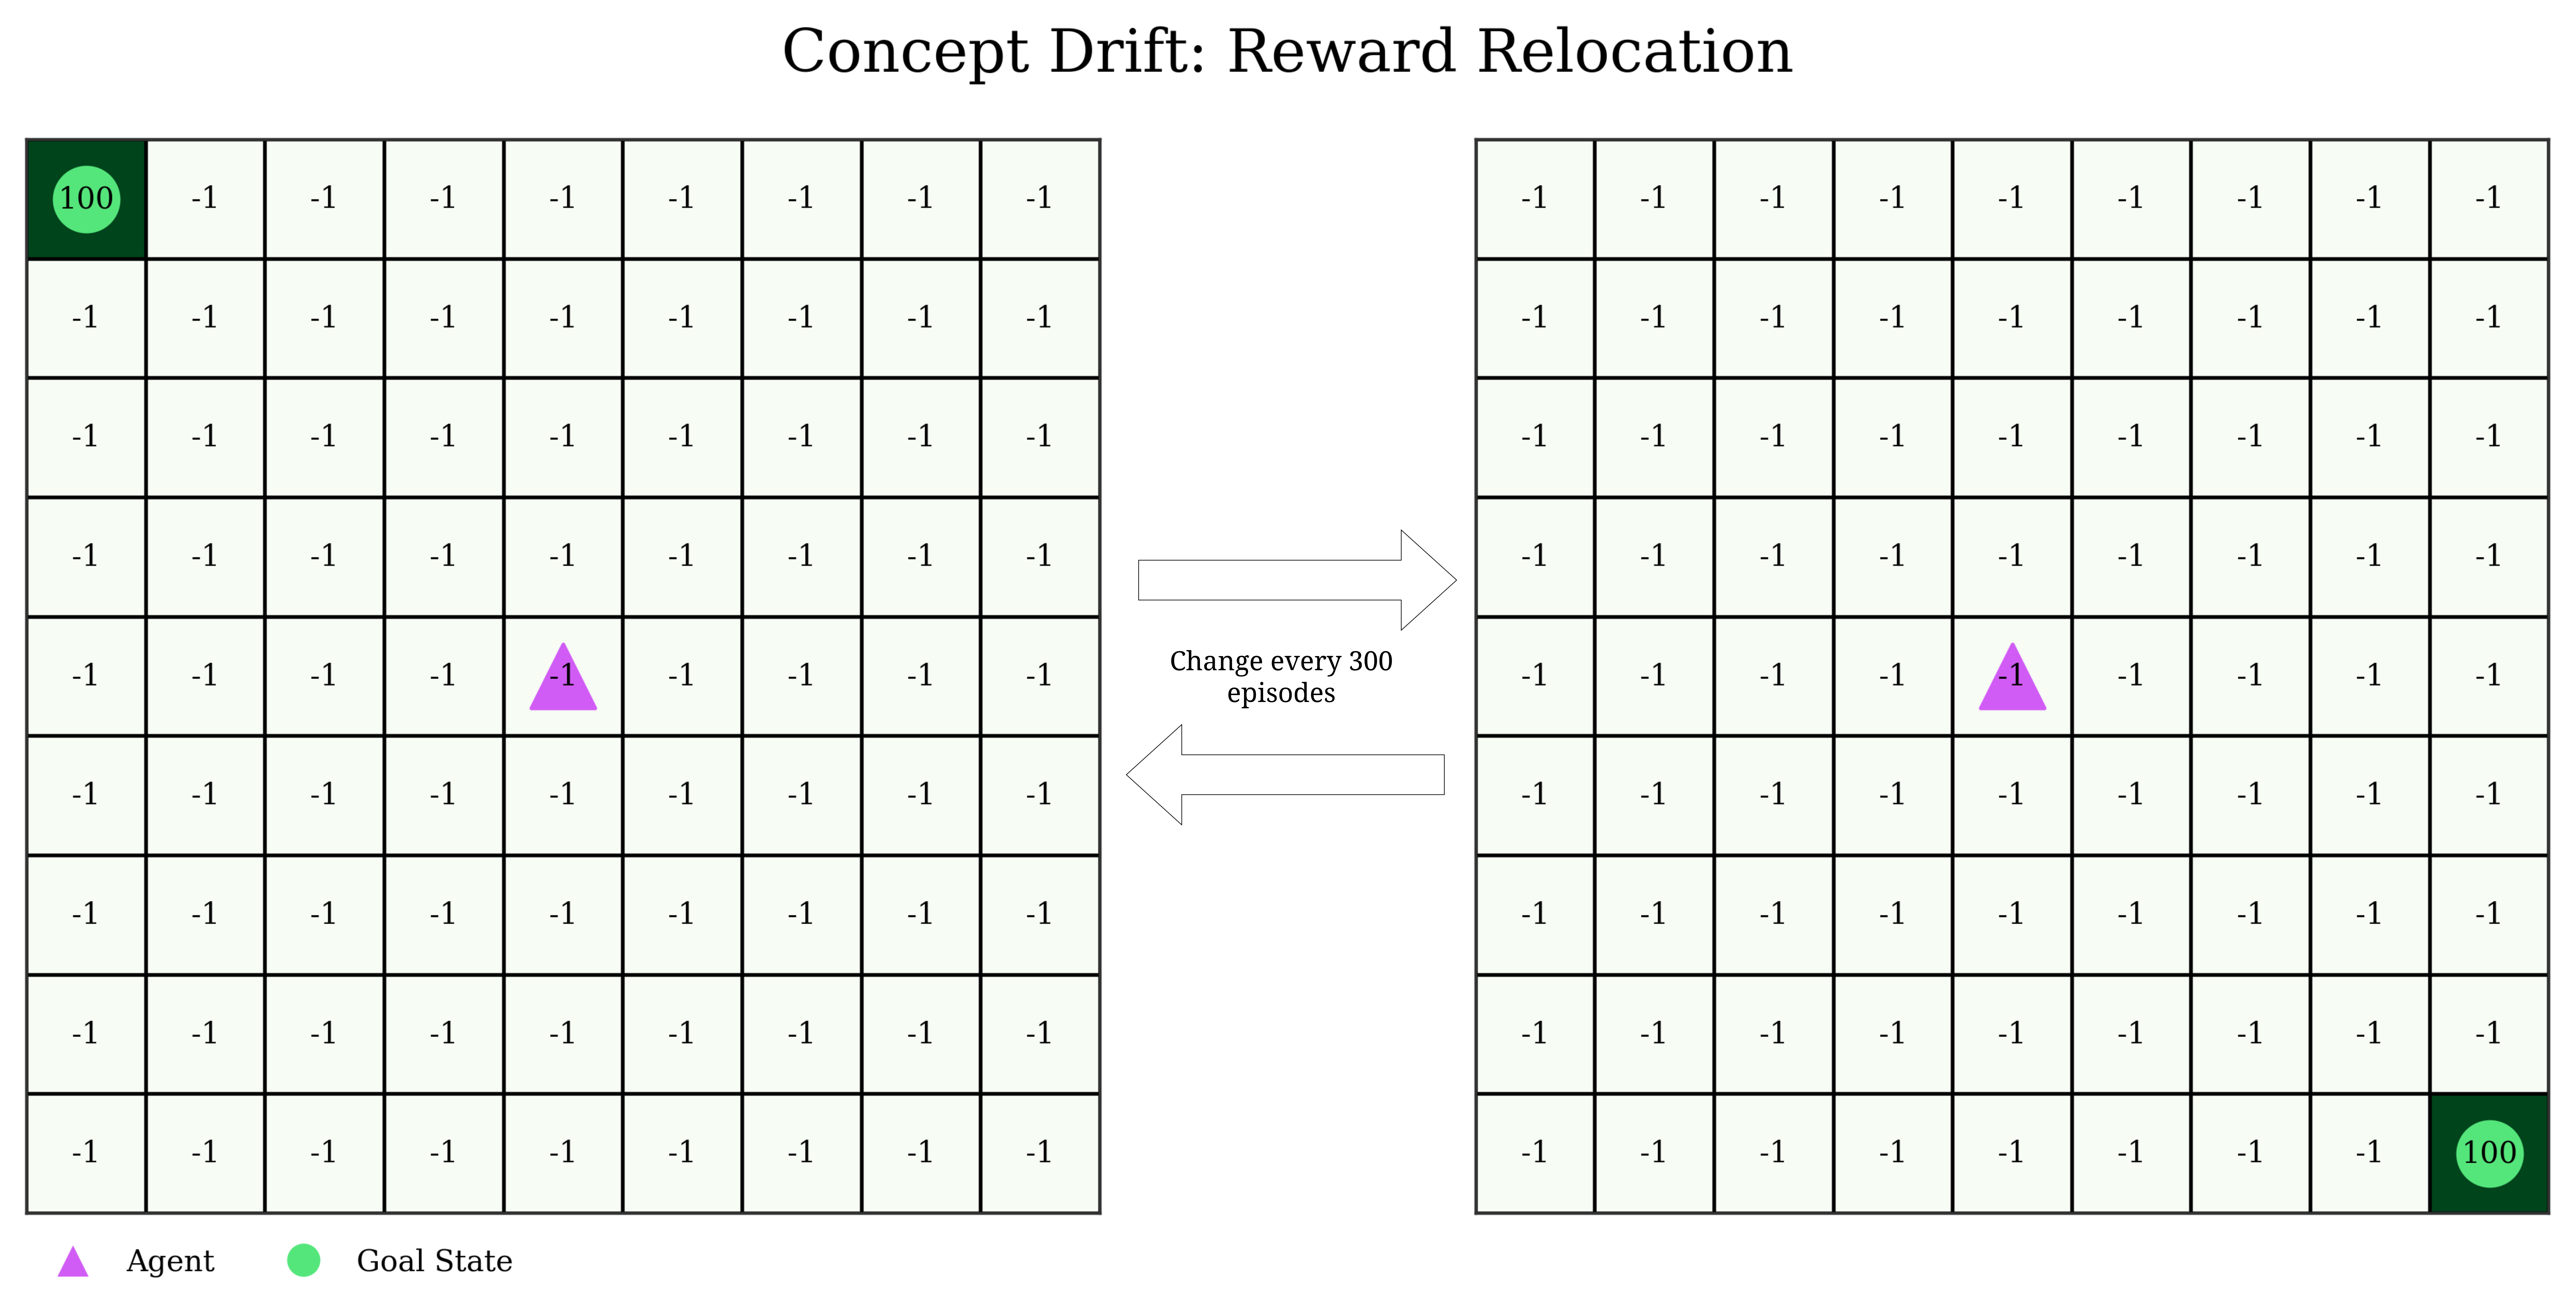
\includegraphics[width=0.9\textwidth]{figures/rewards_change}
    \caption{Non-Stationary Gridworld: Concept drift is induced by relocating the reward. The agent starts at the center and must reach the goal, which alternates between the top-left and bottom-right corners every 300 episodes.}
    \label{fig:r-change}
\end{figure*}

Additionally, we consider a scenario of adding walls to the Gridworld, blocking the agent's movement 
according to its initial set of actions (\fref{fig:q-value-comp2}). For such scenario, we enable the agent 
to  extended its action space by acquiring new actions that provide additional capabilities to the agent 
(\ie jumping). Such situations are common in robotics for modular/evolving 
robots~\cite{eiben20evolving,miras20environmental}, or swarm behavior~\cite{schranz20swarm} where 
robots acquire new capabilities due to the physical attachment of parts, the possibility of combining 
actions with nearby robots, or the transfer of responsibilities/behavior between robots. Whichever the 
case may be, the agent is expected to adapt to these changes and efficiently adjust its policy using 
the newly acquired behavior.


\endinput

